% Mobile-C Library 

%%%%%%%%%%%%%%%%%%%%%%%%%%%%%%%%%%%%%%%%%%%%%%%%%%%%%%%%%%%%%%%%%%%%%%
% Preamble {{{
%\documentclass[11pt]{article}
\documentclass[11pt]{report}
\usepackage{varioref}
\usepackage{times,verbatim,fancyheadings,makeidx}
\usepackage{moreverb}
%\usepackage{psfig}
\usepackage[pdftex]{hyperref}
\usepackage{hypcap}
\usepackage{fullpage}
\usepackage{amssymb,amsmath}
\usepackage{graphicx}
\usepackage{program}
%\headrulewidth 0.0pt
%\hoffset=-0.0625in
%\voffset=0pt
\setlength{\textheight}{9in}
\setlength{\textwidth}{6.5in}
\topmargin=0.05in
\makeindex
% }}} Preamble
%%%%%%%%%%%%%%%%%%%%%%%%%%%%%%%%%%%%%%%%%%%%%%%%%%%%%%%%%%%%%%%%%%%%%%

%%%%%%%%%%%%%%%%%%%%%%%%%%%%%%%%%%%%%%%%%%%%%%%%%%%%%%%%%%%%%%%%%%%%%%
% Title Page {{{
\begin{document}
\thispagestyle{empty}
\begin{center}
%\includegraphics[width=1.8in]{figure/mobilec_logo.png}


\vspace{0.5in}
{\Huge\sf\bf User's Guide for Programming iMobot} \\
\vspace{2.0in}
{\large\sf\bf\today}
%September 20, 2007
\end{center}

\pagebreak
% }}} Title Page
%%%%%%%%%%%%%%%%%%%%%%%%%%%%%%%%%%%%%%%%%%%%%%%%%%%%%%%%%%%%%%%%%%%%%%

%%%%%%%%%%%%%%%%%%%%%%%%%%%%%%%%%%%%%%%%%%%%%%%%%%%%%%%%%%%%%%%%%%%%%%
% Abstract {{{
%\phantomsection
%\addcontentsline{toc}{chapter}{Abstract}
\begin{abstract} 
This user's guide describes how to control an iMobot robotic module.

\end{abstract}
\pagebreak
% Abstract }}}
%%%%%%%%%%%%%%%%%%%%%%%%%%%%%%%%%%%%%%%%%%%%%%%%%%%%%%%%%%%%%%%%%%%%%%

%%%%%%%%%%%%%%%%%%%%%%%%%%%%%%%%%%%%%%%%%%%%%%%%%%%%%%%%%%%%%%%%%%%%%%
% Table of Contents {{{
\pagenumbering{roman}
\setcounter{page}{1}
\tableofcontents
\pagebreak
% }}} Table of Contents
%%%%%%%%%%%%%%%%%%%%%%%%%%%%%%%%%%%%%%%%%%%%%%%%%%%%%%%%%%%%%%%%%%%%%%

%%%%%%%%%%%%%%%%%%%%%%%%%%%%%%%%%%%%%%%%%%%%%%%%%%%%%%%%%%%%%%%%%%%%%%
% Part 1 {{{
\pagenumbering{arabic}
\setcounter{page}{1}
\pagebreak
% }}} Part 1 
%%%%%%%%%%%%%%%%%%%%%%%%%%%%%%%%%%%%%%%%%%%%%%%%%%%%%%%%%%%%%%%%%%%%%%

%%%%%%%%%%%%%%%%%%%%%%%%%%%%%%%%%%%%%%%%%%%%%%%%%%%%%%%%%%%%%%%%%%%%%%
% Introduction {{{
%\pagenumbering{arabic}
%\setcounter{page}{1}
%\pagestyle{fancy}
%\chapter{Introduction}
%\pagebreak
% }}} Introduction
%%%%%%%%%%%%%%%%%%%%%%%%%%%%%%%%%%%%%%%%%%%%%%%%%%%%%%%%%%%%%%%%%%%%%%

\chapter{Getting Started}
This short guide will enable you to run the provided demo program,
``simple.cpp'', on the iMobot.
\begin{enumerate}
\item Download and install a VNC client
  \begin{itemize}
  \item For Windows, you may download and install TightVNC from \texttt{http://www.tightvnc.com}.
  \item For Mac OS X, you may download and install Chicken of the VNC from\\
  \texttt{http://sourceforge.net/projects/cotvnc/}
  \end{itemize}
\item Log in to the imobot with a VNC client. 
\item Connect to the iMobot with your VNC client. The iMobot will create an ad-hoc network
called "imobot" by default upon startup. Connect to the ad-hoc network, and connect
to the iMobot's IP address, which is 192.168.0.1 by default.
\item Open and execute the demo program.
  \begin{enumerate}
  \item Copy the demo program to your home directory with the command\\
  \texttt{cp /usr/local/ch/package/chimobot/demos/simple.cpp \textasciitilde/}
  \item Open the demo program with ChIDE. You may left click on the desktop to open the menu, and select \texttt{Applications -> Accessories -> ChIDE}.
  \item Click on \texttt{File -> Open} within ChIDE and open the program, \texttt{simple.cpp}. 
  \item Click on the ``Run'' button, located near the top right of the ChIDE Window. The robot should now run the program.
  \end{enumerate}
\end{enumerate}

\chapter{Graphical Control Interface}
\begin{figure}
\begin{center}
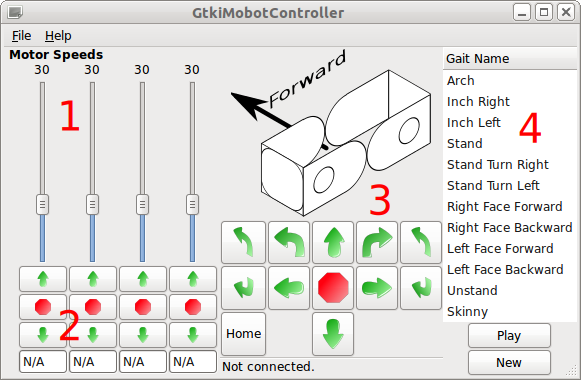
\includegraphics[width=4in]{gui_screenshot.png}
\caption{\label{fig:gui}The iMobot Graphical Control Interface.}
\end{center}
\end{figure}
The iMobot comes with a graphical control interface for controlling the iMobot.
The control interface is able to perform simple locomotion tasks, and can be
used to determine the joint angles of the iMobot. A screenshot of the interface
is shown in Figure \ref{fig:gui}.

The graphical interface can be found in the application menu of the iMobot. Once
a VNC connection to the iMobot has been established, simply left click on the
desktop to bring up the menu, and select the item \texttt{Applications ->
Accessories -> iMobot Controller}. Once the controller starts, it needs to be
initialized in order to establish communication with the motor controllers.
This is done by clicking on \texttt{File -> Init Local I2C Bus}. Ensure that 
the application is connected by ensuring that the status bar at the bottom of the
application displays ``Connected''. 

The graphical interface is composed of six basic components, as shown in
Figure \ref{fig:gui}. There are three components on the top half of the
interface, and three on the bottom half. Each component is discussed in
detail in the following subsections.

\subsection{The iMobot Diagram and ``Move To Zero'' Button}
The first section of the GUI located on the top left of the interface
displays a schematic diagram of the iMobot, displaying motor positions.
Underneath the diagram, there is a large button with the text 
``Move To Zero''. When clicked, this button will command the connected
iMobot to rotate all of its joints to a flat ``Zero'' position.

\subsection{Individual Joint Control}
The second section, located at the top-middle section of the interface,
is the ``Individual Joint Control'' section. These buttons command the
iMobot to move individual joints. When the up or down arrows are clicked,
the iMobot begins to move the corresponding joint in either the positive,
or negative direction. The joint will continue to move until the stop 
button, located between the up and down arrows, is clicked. 

\subsection{Rolling Control}
This section contains buttons for controlling the iMobot as a 
two wheeled mobile robot. The up and down buttons cause the iMobot to
roll forward or backward. The left and right buttons cause the iMobot 
to rotate towards the left, or towards the right. The stop button in the
middle causes the iMobot to stop where it is.

\subsection{Joint Speeds}
The ``Joint Speeds'' section, located at the bottom left of the interface,
displays and controls the current joint speeds of the iMobot. Joint speeds
are a value between 0 and 1, with 1 meaning maximum joint power, and 0
meaning zero joint power. The speed may be set by sliding the vertical 
sliders to the desired positions. 

\subsection{Joint Positions}
This section, located in the bottom-middle of the interface, is used to display
and control the positions of each of the four
joints of a iMobot. The joint positions are displayed in the numerical
text located above each vertical slider. The displayed joint positions are in
units of degrees.  There are two methods to control
the joints using this interface.

The first method of controlling the joints is by using the vertical sliders.
Each vertical slider's position represents a joint's angle. The sliders for the
two end joints vary from -180 degrees to 180 degrees, representing one complete
rotation. The angles for the two body joints vary from -90 to 90 degrees. When
the position of the slider is moved, the iMobot will move its joints to match the 
sliders. 

The second method for moving the joints is by entering the exact angles for the
joints. Below each of the four sliders lies a text entry box. Values in degrees
may be typed into each of the four entry boxes. When the button on the lower
right of the section labeled ``Move'' is clicked, the iMobot will move its joints
to match the values typed into the boxes. If no value is typed into a box, that 
joint will not move.

\subsection{Motions}
This section, located on the bottom right of the interface, contains a set of
preprogrammed motions for the iMobot. To execute a preprogrammed motion, simply
click on the name of the motion you wish to execute, and then click the button
labeled ``Play''.


%%%%%%%%%%%%%%%%%%%%%%%%%%%%%%%%%%%%%%%%%%%%%%%%%%%%%%%%%%%%%%%%%%%%%%
% SUB: Overview of Sample Application Programs {{{
\chapter{Overview of Sample Application Programs}
\subsection{\texttt{simple.cpp} : A Simple Bare-Bones Demo}
The following program is a simple program which moves some joints on the iMobot
before initializing the robot to listen for incoming Bluetooth commands.
\subsubsection{simple.cpp \label{subsec:simple.cpp}}
\listinginput{1}{../demos/simple_cpp/simple.cpp}
\subsubsection{Explanation of simple.cpp}
\begin{itemize}
\item 
\begin{verbatim}
  CiMobot robot;
\end{verbatim}
This line declares the \texttt{robot} object, which represents the
capabilities of the iMobot module. iMobot modules are represented by
the \texttt{CiMobot} type. This object contains various member
functions which may be executed by the user.
\item 
\begin{verbatim}
  robot.moveToZero();
\end{verbatim}
These commands command the iMobot to move all motors to their zero positions
and wait until the motion is finished.
\item 
\begin{verbatim}
  robot.moveTo(90, 0, 0, 90);
\end{verbatim}
These lines instruct the robot to rotate the faceplates, which are the first
and fourth joints, by 90 degrees. 
\item 
\begin{verbatim}
  robot.moveTo(0, 0, 0, 0);
\end{verbatim}
The previous line causes the iMobot to move the first and fourth joints back to
their original position.
\end{itemize}

\subsection{\texttt{bluetoothListener.cpp} : A Demo That Receives and Executes
Bluetooth Commands}
The following program is a bare-bones demo program which initializes the iMobot's
Bluetooth listening capabilities. The program sets up the iMobot so that Bluetooth
enabled devices can connect to and control the iMobot remotely. 
\subsubsection{bluetoothListener.cpp}
\listinginput{1}{../demos/bluetoothListener/bluetoothListener.cpp}
\subsubsection{Explanation of \texttt{bluetoothListener.cpp}}
\begin{itemize}
\item 
\begin{verbatim}
  CiMobot robot;
  int bluetoothChannel = 20; // Default channel
\end{verbatim}
Similar to the previous demo, the first line declares a \texttt{CiMobot} object
called \texttt{robot}. The second line declares an integer variables called 
\texttt{bluetoothChannel}, which is initialized to a value of 20. The 
variable \texttt{bluetoothChannel} represents the channel to listen on
for incoming bluetooth connections.
\item
\begin{verbatim}
  robot.setJointSpeed(IMOBOT_JOINT1, 0.50);
  robot.setJointSpeed(IMOBOT_JOINT2, 0.50);
  robot.setJointSpeed(IMOBOT_JOINT3, 0.50);
  robot.setJointSpeed(IMOBOT_JOINT4, 0.50);
\end{verbatim}
These lines of code set the motor speeds for all four motors to a value of
\texttt{0.50}, or 50\% speed.
\item
\begin{verbatim}
  robot.initListenerBluetooth(bluetoothChannel);
\end{verbatim}
This line initializes the iMobot's Bluetooth listening service. 
\item
\begin{verbatim}
  robot.listenerMainLoop();
\end{verbatim}
This function blocks indefinitely, allowing the iMobot to handle any number of Bluetooth
commands from the remote device. The \texttt{listenerMainLoop()} will return if the
``Quit'' command is sent to the iMobot from the remote device.
\end{itemize}

This demo enables an iMobot to accept bluetooth connections from the corresponding
MoBot library, called \texttt{CMobot}. Please refer to the MoBot documentation
for instructions on how to connect to and control a MoBot remotely via Bluetooth.

%%%%%%%%%%%%%%%%%%%%%%%%%%%%%%%%%%%%%%%%%%%%%%%%%%%%%%%%%%%%%%%%%%%%%%
% SUB: Execution of Sample Applications {{{
%\section{Execution of Sample Applications}
%%%%%%%%%%%%%%%%%%%%%%%%%%%%%%%%%%%%%%%%%%%%%%%%%%%%%%%%%%%%%%%%%%%%%%
% Appendix {{{
\appendix
\chapter{Data Types, Macros, and Constants}
\section{Data Types}
There are data types which are used by the MoBot library to represent 
certain values, such as joint id's and motor directions.

\begin{tabular}{p{3.5cm}p{7cm}} \hline 
Data Type& Description \\
\hline 
\texttt{mobotJointId\_t} & An enumerated value that indicates a MoBot joint. \\
\texttt{mobotJointState\_t} & The current state of a MoBot joint. \\
\texttt{mobotJointDirection\_t} & The current motion direction of a MoBot joint. 
\end{tabular}

\subsection{\label{sec:mobotJointId_t}\texttt{mobotJointId\_t}}
This datatype is an enumerated type used to identify a joint on the MoBot. Valid
values for this type are:
\begin{verbatim}
typedef enum mobot_joints_e {
  MOBOT_JOINT1 = 1,
  MOBOT_JOINT2 = 2,
  MOBOT_JOINT3 = 3,
  MOBOT_JOINT4 = 4
} mobotJointId_t;
\end{verbatim}
The joints are enumerated in order from one side of the MoBot to the other. Joints 1 and 4
are faceplate joints, and joints 2 and 3 are body joints.

\subsection{\label{sec:mobotJointState_t}\texttt{mobotJointState\_t}}
This datatype is an enumerated type used to designate the current 
movement state of a joint. Valid values are:
\begin{itemize}
\item \texttt{MOBOT\_JOINT\_IDLE}: This value indicates that the joint is not moving.
\item \texttt{MOBOT\_JOINT\_MOVING}: This value indicates that the joint is currently moving.
\item \texttt{MOBOT\_JOINT\_GOALSEEK}: This value indicates that the joint is currently moving
  towards a predefined goal.
\end{itemize}

\subsection{\label{sec:mobotJointDirection_t}\texttt{mobotJointDirection\_t}}
This datatype designates a MoBot joint's commanded direction of travel. Valid values
are
\begin{itemize}
\item \texttt{MOBOT\_NEUTRAL}: There is no predesignated direction for the
joint. If the joint is commanded to move to a specific location, the MoBot will
decide the best direction to move the joint in order to achieve the goal with
the smallest motion.
\item \texttt{MOBOT\_FORWARD}: Move the joint in the direction which increases its 
angular position.
\item \texttt{MOBOT\_BACKWARD}: Move the joint in the direction which decreases
its angular position.
\end{itemize}

\section{Macros}

\subsection{\texttt{MoBot\_joints\_t}}
\index{MoBot\_joints\_t}
The data type \texttt{MoBot\_joints\_t} contains the following macro datatypes.\\

\index{IMOBOT\_JOINT1}
\index{IMOBOT\_JOINT2}
\index{IMOBOT\_JOINT3}
\index{IMOBOT\_JOINT4}
\begin{tabular}{p{3cm}p{7cm}} \hline 
Value & Description \\
\hline 
\texttt{IMOBOT\_JOINT1} & Joint number 1 on the MoBot, which is a faceplate joint. \\
\texttt{IMOBOT\_JOINT2} & Joint number 2 on the MoBot, which is a body joint. \\
\texttt{IMOBOT\_JOINT3} & Joint number 3 on the MoBot, which is a body joint. \\
\texttt{IMOBOT\_JOINT3} & Joint number 4 on the MoBot, which is a faceplate joint. 
\end{tabular}

\subsection{\texttt{MoBot\_joint\_direction\_t}}
\index{MoBot\_joint\_direction\_t}
The data type \texttt{MoBot\_joint\_direction\_t} indicates the commanded direction 
of a joint on the MoBot.

\index{IMOBOT\_NEUTRAL}
\index{IMOBOT\_FORWARD}
\index{IMOBOT\_BACKWARD}
\begin{tabular}{p{3cm}p{7cm}} \hline 
Value & Description \\
\hline 
\texttt{IMOBOT\_NEUTRAL} & This value indicates automatic direction control for a joint. 
The MoBot will choose the best direction to attain the commanded joint position. \\
\texttt{IMOBOT\_FORWARD} & Move the joint in the forward direction. \\
\texttt{IMOBOT\_BACKWARD} & Move the joint in the backward direction. \\
\end{tabular}

\chapter{iMobot API}
\lhead{libimobot API Documentation}
\noindent
The header file {\bf libimobot.h} defines all the data types, macros 
and function prototypes for the iMobot API library. The header file
declares a class called \texttt{CiMobot} which contains member functions which
may be used to control the robot.

\begin{table}[!hp]
\capstart
\begin{center}
\caption{CiMobot Member Functions.}
\begin{tabular}{p{58 mm}p{97 mm}}
%\begin{tabular}{ll}
\hline
Function & Description \\
\hline
%\texttt{pose()} \dotfill & Pose multiple joints of the iMobot. \\
\texttt{CiMobot()} \dotfill & The CiMobot constructor function. This function
is called automatically and should not be called explicitly. \\
\texttt{\textasciitilde CiMobot()} \dotfill & The CiMobot destructor function. This function
is called automatically and should not be called explicitly. \\
& \\
\texttt{getJointAngle()} \dotfill & Gets a joint's angle. \\
\texttt{getJointAngles()} \dotfill & Gets all joint angles. \\
\texttt{getMotorSpeed()} \dotfill & Gets a motor's speed. \\
\texttt{initListenerBluetooth()} \dotfill & Initialize the Bluetooth module to
listen for incoming commands. \\
\texttt{isBusy()} \dotfill & See if the robot is currently moving. \\
\texttt{listenerMainLoop()} \dotfill & Main execution loop for the Bluetooth listener. \\
\texttt{moveJoint()} \dotfill & Move a joint of the imobot by some amount from its current location. \\
\texttt{moveWait()} \dotfill & Wait until all motors have stopped moving. \\
\texttt{poseJoint()} \dotfill & Pose a single joint of the iMobot. \\
\texttt{setMotorDirection()} \dotfill & Set the motor direction of a motor. Set
to "0" for automatic direction, "1" for forward, and "2" for reverse. \\
\texttt{setMotorSpeed()} \dotfill & Sets a motor's speed. \\
\texttt{stop()} \dotfill & Stop all currently executing motions of the iMobot. \\
\texttt{terminate()} \dotfill & Terminate the robotic control. \\
\texttt{waitMotor()} \dotfill & Wait until the specified motor has stopped moving. \\
\hline
\end{tabular}
\end{center}
\label{mobilec_api_cbinary}
\end{table}

\newpage
\noindent
\vspace{5pt}
\rule{4.5in}{0.015in}\\
\noindent
{\LARGE \texttt{CMobot::getJointAngle()}\index{getJointAngle()}}\\
%\phantomsection
\addcontentsline{toc}{section}{getJointAngle()}

\noindent
{\bf Synopsis}\\
\begin{verbatim}
#include <mobot.h>
int CMobot::getJointAngle(mobotJointId_t id, double &position);
\end{verbatim}

\noindent
{\bf Purpose}\\
Connect to a remote MoBot via Bluetooth.\\

\noindent
{\bf Return Value}\\
The function returns 0 on success and non-zero otherwise.\\

\noindent
{\bf Parameters}\\
\vspace{-0.1in}
\begin{description}
\item               
\begin{tabular}{p{15 mm}p{105 mm}}
\texttt{id} & The joint number to wait for. This is an enumerated type 
discussed in Section \ref{sec:mobotJointId_t} on page
\pageref{sec:mobotJointId_t}.\\
\texttt{position} & A variable to store the current position of the MoBot
motor. The contents of this variable will be overwritten with a value that
represents the motor's angle in degrees.  \\
\end{tabular}
\end{description}

\noindent
{\bf Description}\\
This function gets the current motor position of a MoBot's motor. The
position returned is in units of degrees and is accurate to roughly $\pm0.1$
degrees. \\

\noindent
{\bf Example}\\
\noindent

\noindent
{\bf See Also}\\
\texttt{connectWithAddress()}

%\CPlot::\DataThreeD(), \CPlot::\DataFile(), \CPlot::\Plotting(), \plotxy().\\

\pagebreak
\noindent
\vspace{5pt}
\rule{4.5in}{0.015in}\\
\noindent
{\LARGE \texttt{CMobot::getJointAngles()}\index{CMobot::getJointAngles()}}\\
{\LARGE \texttt{CMobot::getJointAnglesAbs()}\index{CMobot::getJointAnglesAbs()}}\\
%\phantomsection
\addcontentsline{toc}{section}{getJointAngles()}

\noindent
{\bf Synopsis}
\vspace{-8pt}
\begin{verbatim}
#include <mobot.h>
int CMobot::getJointAngles(
    double &angle1,
    double &angle2,
    double &angle3,
    double &angle4);
int CMobot::getJointAnglesAbs(
    double &angle1,
    double &angle2,
    double &angle3,
    double &angle4);
\end{verbatim}

\noindent
{\bf Purpose}\\
Retrieve a Mobot's current joint angles.\\

\noindent
{\bf Return Value}\\
The function returns 0 on success and non-zero otherwise.\\

\noindent
{\bf Parameters}\\
\vspace{-0.1in}
\begin{description}
\item               
\begin{tabular}{p{15 mm}p{145 mm}}
\texttt{angle1} & A variable to store the current angle of the mobot
motor. The contents of this variable will be overwritten with a value that
represents the motor's angle in degrees.  \\
\texttt{angle2} & ...  \\
\texttt{angle3} & ...  \\
\texttt{angle4} & ...  \\
\end{tabular}
\end{description}

\noindent
{\bf Description}\\
This function gets the current motor angles of a Mobot's motors. The
angle returned is in units of degrees and is accurate to roughly $\pm0.17$
degrees. 

The function \texttt{getJointAngles()} always returns an angle between -180 and
+180 degrees. The \texttt{getJointAnglesAbs()} function, however, gets the total
angle the joint has turned since the mobot has been powered on. For instance, 
if the faceplate joint 1 has been rotated two full rotations after initial power up,
  the function \texttt{getJointAngles()} will report that the joint is at angle 0,
  whereas the function \texttt{getJointAnglesAbs()} will report that the joint
  angle is 720 degrees.
\\

\noindent
{\bf Example}\\
\noindent

\noindent
{\bf See Also}\\

%\CPlot::\DataThreeD(), \CPlot::\DataFile(), \CPlot::\Plotting(), \plotxy().\\

\pagebreak
\input{api/getMotorSpeed}
\pagebreak
\noindent
\vspace{5pt}
\rule{6.5in}{0.015in}
\noindent
{\LARGE \texttt{CiMobot::initListenerBluetooth()}\index{initListenerBluetooth()}}\\
\phantomsection
\addcontentsline{toc}{section}{initListenerBluetooth()}

\noindent
{\bf Synopsis}\\
\begin{verbatim}
#include <imobot.h>
int CiMobot::initListenerBluetooth(int channel);
\end{verbatim}

\noindent
{\bf Purpose}\\
Initialize the bluetooth listening service to process incoming bluetooth commands.\\

\noindent
{\bf Return Value}\\
The function returns 0 on success and non-zero otherwise.\\

\noindent
{\bf Parameters}
\vspace{-0.1in}
\begin{description}
\item               
\begin{tabular}{p{20 mm}p{145 mm}}
\texttt{channel} & The bluetooth channel to listen on. The default value is "20". \\
\end{tabular}
\end{description}

\noindent
{\bf Description}\\
This function initialized the iMobot's bluetooth listening service so that it may process incoming Bluetooth commands. If this function is not called, the iMobot will not listen to any bluetooth commands.

\noindent
{\bf Example}\\
See the sample program in Section \ref{subsec:simple.cpp} on page \pageref{subsec:simple.cpp}.
\noindent

\noindent
{\bf See Also}\\
\texttt{moveWait(), waitMotor()}

%\CPlot::\DataThreeD(), \CPlot::\DataFile(), \CPlot::\Plotting(), \plotxy().\\

\pagebreak
\noindent
\vspace{5pt}
\rule{6.5in}{0.015in}
\noindent
{\LARGE \texttt{CiMobot::isBusy()}\index{isBusy()}}\\
\phantomsection
\addcontentsline{toc}{section}{isBusy()}

\noindent
{\bf Synopsis}\\
\begin{verbatim}
#include <imobot.h>
int CiMobot::isBusy();
\end{verbatim}

The usage of this function is identical to the
\texttt{CMobot::isBusy()} function for the MoBot. Please refer
to the MoBot documentation for \texttt{CMobot::isBusy} for
detailed usage documentation.


\pagebreak
\noindent
\vspace{5pt}
\rule{6.5in}{0.015in}
\noindent
{\LARGE \texttt{CiMobot::listenerMainLoop()}\index{listenerMainLoop()}}\\
\phantomsection
\addcontentsline{toc}{section}{listenerMainLoop()}

\noindent
{\bf Synopsis}\\
\begin{verbatim}
#include <imobot.h>
int CiMobot::listenerMainLoop();
\end{verbatim}

\noindent
{\bf Purpose}\\
Put the iMobot into Bluetooth listening mode.\\

\noindent
{\bf Return Value}\\
The function returns 0 on success and non-zero otherwise.\\

\noindent
{\bf Description}\\
This function puts the iMobot into Bluetooth listening mode. This function will
not return until it receives a Bluetooth "quit" command.

\noindent
{\bf Example}\\
See the sample program in Section \ref{subsec:simple.cpp} on page \pageref{subsec:simple.cpp}.
\noindent

\noindent
{\bf See Also}\\

%\CPlot::\DataThreeD(), \CPlot::\DataFile(), \CPlot::\Plotting(), \plotxy().\\

\pagebreak
\noindent
\vspace{5pt}
\rule{6.5in}{0.015in}
\noindent
{\LARGE \texttt{CiMobot::moveJoint()}\index{moveJoint()}}\\
{\LARGE \texttt{CiMobot::moveJointNB()}\index{moveJointNB()}}\\
\phantomsection
\addcontentsline{toc}{section}{moveJoint()}
\addcontentsline{toc}{section}{moveJointNB()}

\noindent
{\bf Synopsis}\\
\begin{verbatim}
#include <imobot.h>
int CiMobot::moveJoint( double angle1, 
                        double angle2, 
                        double angle3, 
                        double angle4);

int CiMobot::moveJointNB( double angle1, 
                          double angle2, 
                          double angle3, 
                          double angle4);
\end{verbatim}

The usage of these functions are identical to the
\texttt{CMobot::moveJoint()} and \texttt{CMobot::moveJointNB()} functions for the MoBot.
Please refer to the MoBot documentation for \texttt{CMobot::moveJoint()} and
\texttt{CMobot::moveJointNB()} for
detailed usage documentation.


\pagebreak
\noindent
\vspace{5pt}
\rule{4.5in}{0.015in}\\
\noindent
{\LARGE \texttt{CMobot::moveWait()}\index{CMobot::moveWait()}}\\
%\phantomsection
\addcontentsline{toc}{section}{moveWait()}

\noindent
{\bf Synopsis}
\vspace{-8pt}
\begin{verbatim}
#include <mobot.h>
int CMobot::moveWait();
\end{verbatim}

\noindent
{\bf Purpose}\\
Wait for all joints to stop moving.\\

\noindent
{\bf Return Value}\\
The function returns 0 on success and non-zero otherwise.\\

\noindent
{\bf Description}\\
This function is used to wait for all joint motions to finish. Functions such as
\texttt{move()} and \texttt{moveTo()} do not wait for a joint to finish
moving before continuing to allow multiple joints to move at the same time. The
\texttt{moveWait()} function is used to wait for
mobotic motions to complete.

Please note that if this function is called after a motor has been commanded to
turn indefinitely, this function may never return and your program may hang.\\

\noindent
{\bf Example}\\
See the sample program in Section \ref{sec:democode} on page \pageref{sec:democode}.
\noindent

\noindent
{\bf See Also}\\
\texttt{moveWait(), moveJointWait()}

%\CPlot::\DataThreeD(), \CPlot::\DataFile(), \CPlot::\Plotting(), \plotxy().\\

\pagebreak
\noindent
\vspace{5pt}
\rule{6.5in}{0.015in}
\noindent
{\LARGE \texttt{poseJoint()}\index{poseJoint()}}\\
\phantomsection
\addcontentsline{toc}{section}{poseJoint()}

\noindent
{\bf Synopsis}\\
\begin{verbatim}
#include "imobot.h"
int CiMobot::poseJoint(unsigned short id, double angle);
\end{verbatim}

\noindent
{\bf Purpose}\\
Pose a joint on the iMobot.\\

\noindent
{\bf Return Value}\\
The function returns 0 on success and non-zero otherwise.\\

\noindent
{\bf Parameters}
\vspace{-0.1in}
\begin{description}
\item               
\begin{tabular}{p{10 mm}p{145 mm}}
\texttt{id} & The joint number to pose. \\
\texttt{angle} & The desired angle in degrees.
\end{tabular}
\end{description}

\noindent
{\bf Description}\\
This function instructs the iMobot to pose a joint to a certain angle. This
function does not wait for the motion to complete before returning. Thus,
multiple successive calls to this function may be used to pose multiple joints
simultaneously. The \texttt{waitMotor()} or \texttt{moveWait()} functions should
be used if the program should wait for motions to complete before continuing. \\

\noindent
{\bf Example}\\
See the sample program in Section \ref{subsec:simple.cpp} on page \pageref{subsec:simple.cpp}.
\noindent

\noindent
{\bf See Also}\\
\texttt{moveWait(), waitMotor()}

%\CPlot::\DataThreeD(), \CPlot::\DataFile(), \CPlot::\Plotting(), \plotxy().\\

\pagebreak
\noindent
\vspace{5pt}
\rule{4.5in}{0.015in}\\
\noindent
{\LARGE \texttt{CiMobotComms::setMotorDirection()}\index{setMotorDirection()}}\\
%\phantomsection
\addcontentsline{toc}{section}{setMotorDirection()}

\noindent
{\bf Synopsis}\\
\begin{verbatim}
#include <imobotcomms.h>
int CiMobotComms::setMotorDirection(int id, int direction);
\end{verbatim}

\noindent
{\bf Purpose}\\
Set's a motor's direction. In conjunction with \texttt{setMotorSpeed()}, this
function may be used to cause a motor to turn indefinitely.\\

\noindent
{\bf Return Value}\\
The function returns 0 on success and non-zero otherwise.\\

\noindent
{\bf Parameters}
\vspace{-0.1in}
\begin{description}
\item               
\begin{tabular}{p{20 mm}p{145 mm}}
\texttt{id} & The joint number to move. \\
\texttt{direction} & A value indicating the desired direction.
\end{tabular}
\end{description}

\noindent
{\bf Description}\\
This function is used to set a motor's turn direction. Possible values for the
direction are:
\begin{itemize}
\item 0: Automatic direction. This is the default setting. 
\item 1: Forward. If this value is used with a non-zero speed set using the
\texttt{setMotorSpeed()} function, the motor will turn forward indefinitely.
\time 2: Backward. Similar to "1", except the motor will spin backward.
\end{itemize}

\noindent
{\bf Example}\\
\noindent

\noindent
{\bf See Also}\\

%\CPlot::\DataThreeD(), \CPlot::\DataFile(), \CPlot::\Plotting(), \plotxy().\\

\pagebreak
\noindent
\vspace{5pt}
\rule{6.5in}{0.015in}
\noindent
{\LARGE \texttt{CiMobot::setMotorSpeed()}\index{setMotorSpeed()}}\\
\phantomsection
\addcontentsline{toc}{section}{setMotorSpeed()}

\noindent
{\bf Synopsis}\\
\begin{verbatim}
#include <imobot.h>
int CiMobot::setMotorSpeed(unsigned short id, unsigned short speed);
\end{verbatim}

\noindent
{\bf Purpose}\\
Get the speed of a joint on the iMobot.\\

\noindent
{\bf Return Value}\\
The function returns 0 on success and non-zero otherwise.\\

\noindent
{\bf Parameters}
\vspace{-0.1in}
\begin{description}
\item               
\begin{tabular}{p{10 mm}p{145 mm}}
\texttt{id} & The joint number to pose. \\
\texttt{speed} & An unsigned short variable indicating the requested speed.
\end{tabular}
\end{description}

\noindent
{\bf Description}\\
This function is used to set the speed of a joint of an iMobot. Valid speed
values range from 0 to 100.
\noindent
{\bf Example}\\
\noindent

\noindent
{\bf See Also}\\

%\CPlot::\DataThreeD(), \CPlot::\DataFile(), \CPlot::\Plotting(), \plotxy().\\

\pagebreak
\noindent
\vspace{5pt}
\rule{6.5in}{0.015in}
\noindent
{\LARGE \texttt{CiMobot::stop()}\index{stop()}}\\
\phantomsection
\addcontentsline{toc}{section}{stop()}

\noindent
{\bf Synopsis}\\
\begin{verbatim}
#include <imobot.h>
int CiMobot::stop();
\end{verbatim}

The usage of this function is identical to the
\texttt{CMobot::stop()} function for the MoBot.
Please refer to the MoBot documentation for \texttt{CMobot::stop()} for
detailed usage documentation.


\pagebreak
\noindent
\vspace{5pt}
\rule{6.5in}{0.015in}
\noindent
{\LARGE \texttt{terminate()}\index{terminate()}}\\
\phantomsection
\addcontentsline{toc}{section}{terminate()}

\noindent
{\bf Synopsis}\\
\begin{verbatim}
#include "imobot.h"
int CiMobot::terminate();
\end{verbatim}

\noindent
{\bf Purpose}\\
Terminate control of an iMobot.\\

\noindent
{\bf Return Value}\\
The function returns 0 on success and non-zero otherwise.\\

\noindent
{\bf Description}\\
This function releases control of the I2C bus, thus terminating communications
with the iMobot. Only a single program may control the iMobot at the same time. If multiple programs are running, the program that currently has control of the iMobot needs to call the \texttt{terminate()} function before other programs can control the iMobot.

\noindent
{\bf Example}\\
See the sample program in Section \ref{subsec:simple.cpp} on page \pageref{subsec:simple.cpp}.
\noindent

\noindent
{\bf See Also}\\

%\CPlot::\DataThreeD(), \CPlot::\DataFile(), \CPlot::\Plotting(), \plotxy().\\

\pagebreak
\noindent
\vspace{5pt}
\rule{4.5in}{0.015in}\\
\noindent
{\LARGE \texttt{CiMobotComms::waitMotor()}\index{waitMotor()}}\\
%\phantomsection
\addcontentsline{toc}{section}{waitMotor()}

\noindent
{\bf Synopsis}\\
\begin{verbatim}
#include <imobot.h>
int CiMobotComms::waitMotor(int id);
\end{verbatim}

\noindent
{\bf Purpose}\\
Wait for a joint to stop moving.\\

\noindent
{\bf Return Value}\\
The function returns 0 on success and non-zero otherwise.\\

\noindent
{\bf Parameters}
\vspace{-0.1in}
\begin{description}
\item               
\begin{tabular}{p{10 mm}p{145 mm}}
\texttt{id} & The joint number to wait for. \\
\end{tabular}
\end{description}

\noindent
{\bf Description}\\
This function is used to wait for a joint motion to finish. Functions such as
\texttt{poseJoint()} and \texttt{moveJoint()} do not wait for a joint to finish
moving before continuing to allow multiple joints to move at the same time. The
\texttt{waitMotor()} or \texttt{waitMotor()} functions are used to wait for
robotic motions to complete.

Please note that if this function is called after a motor has been commanded to
turn indefinitely, this function may never return and your program may hang.\\

\noindent
{\bf Example}\\
See the sample program in Section \ref{subsec:simple.cpp} on page \pageref{subsec:simple.cpp}.
\noindent

\noindent
{\bf See Also}\\
\texttt{moveWait()}

%\CPlot::\DataThreeD(), \CPlot::\DataFile(), \CPlot::\Plotting(), \plotxy().\\


\pagebreak
% }}} Appendix 
%%%%%%%%%%%%%%%%%%%%%%%%%%%%%%%%%%%%%%%%%%%%%%%%%%%%%%%%%%%%%%%%%%%%%%

%%%%%%%%%%%%%%%%%%%%%%%%%%%%%%%%%%%%%%%%%%%%%%%%%%%%%%%%%%%%%%%%%%%%%%
% Index {{{
\phantomsection
\addcontentsline{toc}{chapter}{Index}
\printindex
% }}} Index 
%%%%%%%%%%%%%%%%%%%%%%%%%%%%%%%%%%%%%%%%%%%%%%%%%%%%%%%%%%%%%%%%%%%%%%
\end{document}
